\textbf{\textcolor{blue}{4.}} Urrutia esta trabajando en un nuevo proyecto para obtener cuentas de detalle de tablas de información, por ejemplo tenemos las siguientes dos tablas:

\begin{center}
    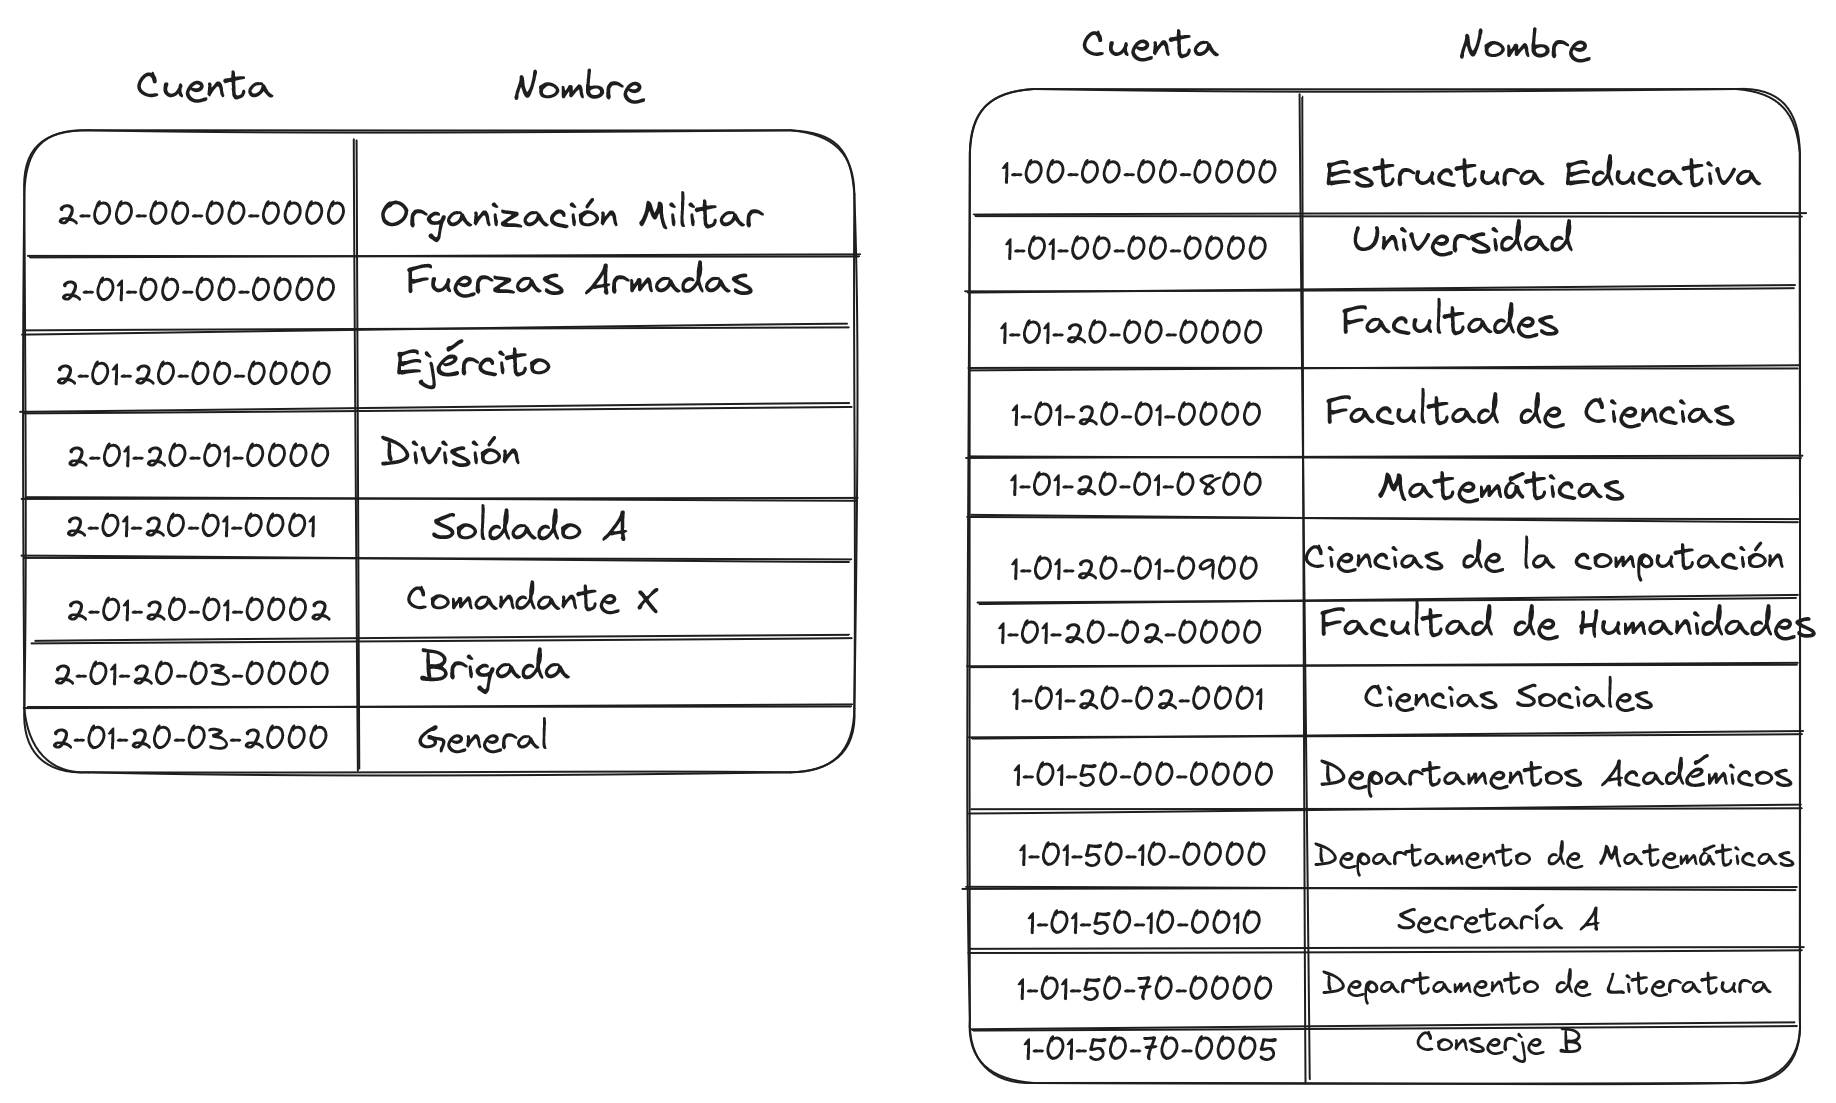
\includegraphics[scale=0.2]{../Image/Tablas.png}
\end{center}
    
Estas tablas contiene información ordenada de formar jerárquica, y a nosotros nos interesaa extraer la información de menor jerarquía pero sin perder el nombre de las cuentas de mayor jerarquía a las que pertenecen, es decir buscamos una tabla como resultado final de esta manera:

\begin{center}
    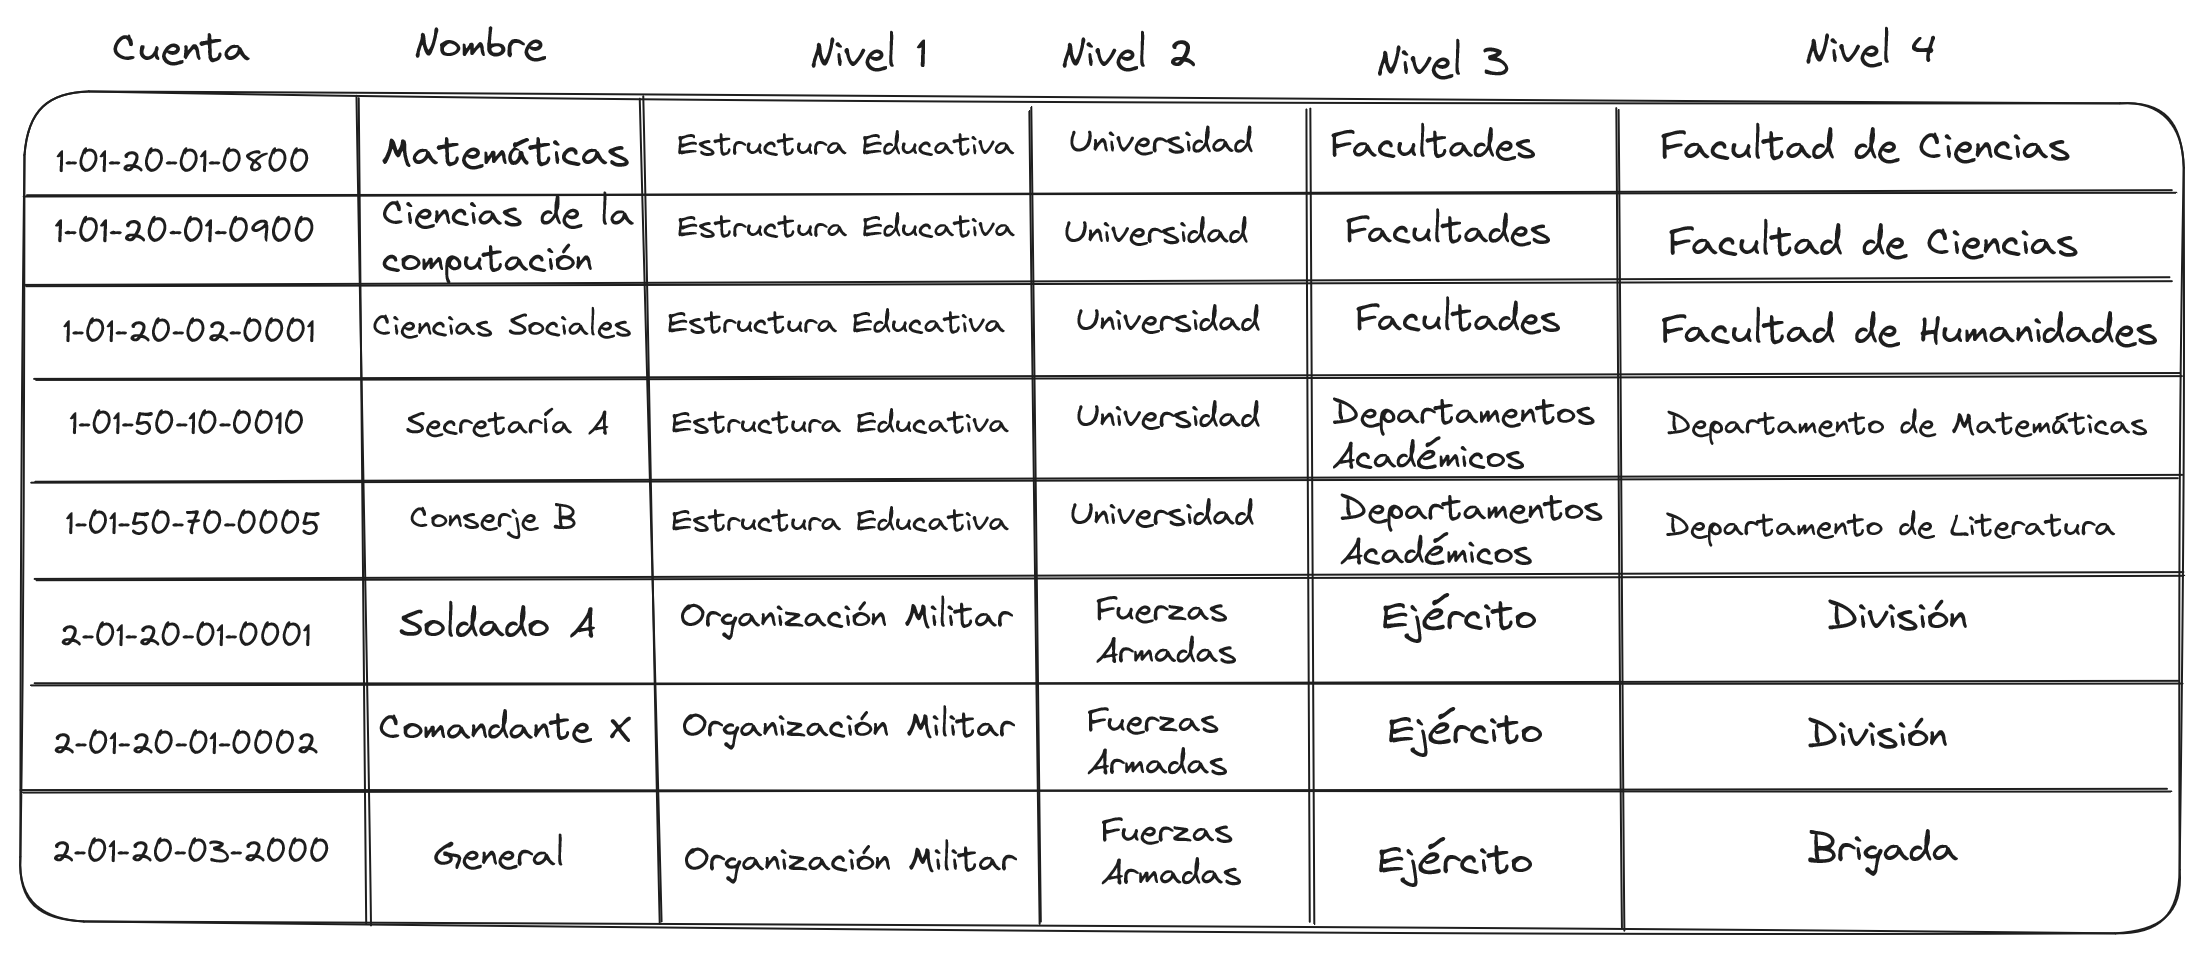
\includegraphics[scale=0.2]{../Image/Resultado.png}
\end{center}

Urrutia se dio cuenta que puede construir un árbol n-ario para resolver de manera fácil este problema basándose en los números de cuenta para construir una llave que le ayudará a decidir si un nodo es hijo o no de otro nodo, hizo un diagrama que representa como debería quedar su árbol n-ario:
\newpage

\begin{center}
    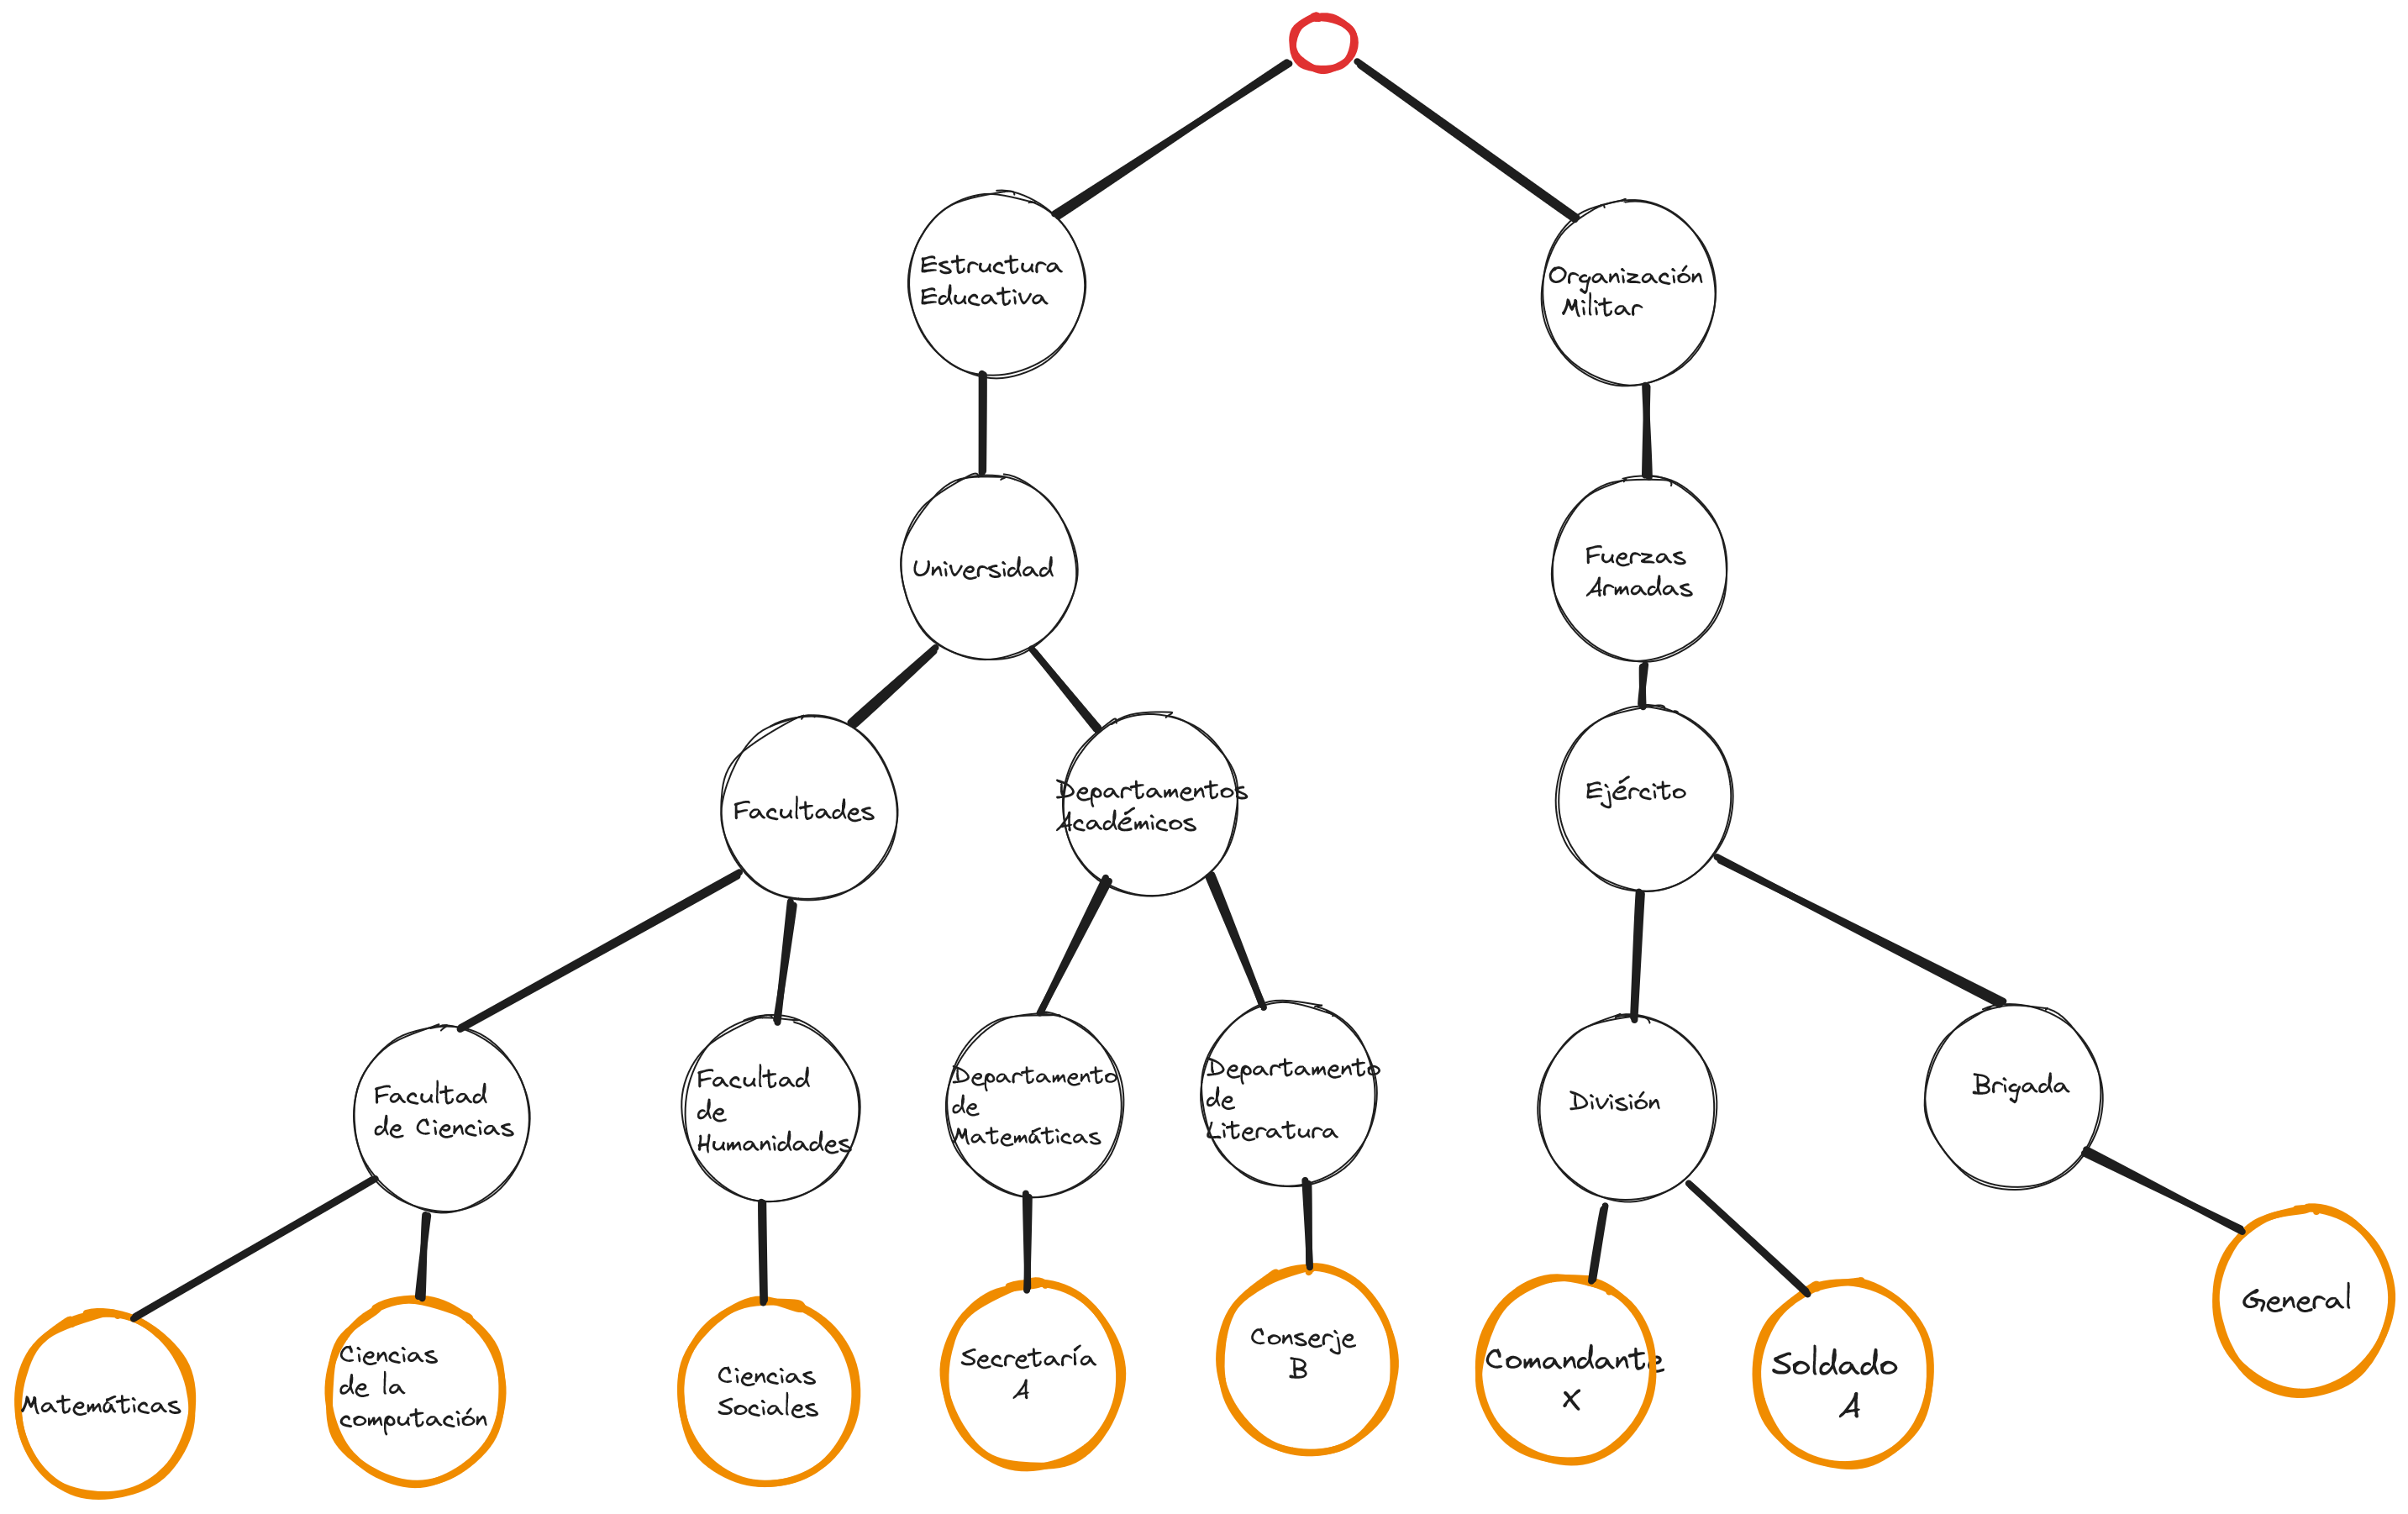
\includegraphics[scale=0.1]{../Image/Arbol.png}
\end{center}

No dibujó los números de cuenta en su diagrama para ahorrar espacio pero cada nodo tiene su número de cuenta. Ahora con ese árbol solo tiene que hacer un recorrido DFS hasta llegar a las hojas para obtener las cuentas de detalle y construir la tabla anterior.

El problema es que Urrutia olvido casi todo su conocimiento de su curso de estructuras de datos de segundo semestre, pero seguramente tu no, así que te pedimos que le ayudes a Urrutia dandole el algoritmo "Inserta" para construir este árbol N-ario, es decir cada nodo puede tener uno o varios hijos, consideraciones a tomar en cuenta es que el nodo raíz es un nodo maestro que no almacena información pero sostiene a los nodos que si la tienen.

Se espera usar tu algoritmo "Inserta" para ir insertando las filas de las tablas iniciales uno por uno en orden jerarquico en forma de nodos, los nodos almacenan los nombres de cuenta y las llaves se basan en los números cuenta separados por un guión pero no necesariamente tienen que ser exactamente iguales.

Hints: Observa como los números de cuenta son grupos separados por guiones, para pasar de un nivel de jerarquía mayor a uno menor se conserva el prefijo y se modifica el sufijo. \\ ¿Que pasaría si por ejemplo convertimos "1-00-00-00-0000" a "1" y "1-01-00-00-0000" a "1-1"? ¿Como sabemos que "1-1" es un número de cuenta de menor jerarquía que "1"? (2 puntos)\newline


$\rhd$\textbf{Solución.} \textit{Inserta}.
\begin{enumerate}
\item Tomemos a nuestra raíz como pivote y no insertemos valor alguno en ella.
\item Los dos hijos de la raíz serán $1$ y $2$, que son los posibles prefijos de las cuentas en ambas tablas.
\item Tenemos un formato X-Y-Z-... Entonces X debe ser $1$ o $2$, Y representará el siguiente nivel y será hijo
de X, luego Z representará un siguiente nivel y será hijo de Y, y así de manera sucesiva.
\item El árbol se comportará como un ``árbol ordenado'' bajo el siguiente criterio: si un nodo tiene 2 o más hijos estos
están dados de izquierda a derecha y de menor a mayor rango (i.e., insertamos 00 a la izquierda de 01 y a su vez 01
quedaría a la izquierda de 20). Así nuestro árbol guarda cierta jerarquía.
\end{enumerate}

¿Que pasaría si por ejemplo convertimos "1-00-00-00-0000" a "1" y "1-01-00-00-0000" a "1-1"? Iniciamos desde la raíz,
bajamos a $1$ (hijo izquierdo de la raíz) y seguimos bajando hacia la izquierda para encontrar "1-00-00-00-0000",
que tendrá una mayor jerarquía que "1-01-00-00-0000" por estar más a la izquierda en su recorrido hacia abajo.\newline

 ¿Como sabemos que "1-1" es un número de cuenta de menor jerarquía que "1"? Por el recorrido en profundidad, pues tenemos que
 movernos más a la derecha que para 1.
\hfill $\lhd$
